\chapter{The funding application}

\section{Motivation of the proposed theme in the current scientific context}

As AI continues to move from cloud environments to edge and embedded platforms, new challenges are emerging related to performance, energy efficiency, and deployment complexity. Running AI models on devices with tight constraints—such as microcontrollers, wearables, or industrial sensors—requires more than just model compression or simplified architectures. It demands a shift in how systems are designed. This project is motivated by the need for a \textbf{co-design approach}, where AI algorithms are developed in close coordination with the hardware and software systems that will execute them.

Recent research highlights the limitations of treating AI development and deployment as separate stages. Lin et al. (2023) demonstrate that algorithm-hardware co-design can significantly reduce energy use and latency in embedded systems compared to post-training optimizations~\cite{lin2023codesign}. Similarly, Hao et al. (2020) show how tailoring neural network structures to specific hardware features, such as memory hierarchies or instruction sets, can lead to substantial performance gains without requiring additional resources~\cite{hao2020fpga}.

However, many current solutions remain fragmented—focused either on model compression or runtime optimization, but rarely both in an integrated manner. This project addresses that gap by proposing a \textbf{modular, full-stack co-design framework}. It is intended to guide the joint development of AI models and embedded system infrastructure, from architecture selection to real-time scheduling, memory management, and secure inference.

\subsection{Scientific Motivation}

The motivation behind this project lies in four key areas where conventional design practices fall short:

\begin{itemize}
    \item \textbf{Latency and Determinism:} Many embedded AI applications—such as fault detection in industrial equipment or gesture recognition in wearables—require sub-millisecond response times. These constraints cannot be met by conventional AI toolchains designed for cloud-scale inference.

    \item \textbf{Resource Efficiency:} Edge devices operate under strict limitations in RAM, compute, and power. Co-design enables the development of models and runtimes that are optimized specifically for these environments, avoiding unnecessary overhead.

    \item \textbf{Security and Privacy:} On-device inference improves data privacy but introduces new risks. Secure storage of AI models, runtime integrity checks, and encrypted communication must be considered part of the design—not added later.

    \item \textbf{Adaptability:} AI models and hardware platforms evolve quickly. A reusable co-design methodology allows faster retargeting of applications to new devices without rewriting software from scratch.
\end{itemize}

The proposed work builds directly on recent advances in edge AI deployment. For example, Zhang et al. (2024) emphasize the need for joint optimization of model structure and system constraints when deploying large models on edge devices~\cite{zhang2024edge}. Atienza (2023) similarly advocates for co-design strategies that take into account both computational efficiency and communication needs in constrained environments~\cite{atienza2023codesign}.

\section{Objectives, methodology and work plan}

\subsection{Concrete Objectives}
Edge artificial-intelligence is at an inflection point: deep-learning models that once required the scale of cloud servers are now expected to operate on milliwatt-class microcontrollers embedded in every segment of the Internet of Things, from environmental sensors that guard biodiversity in remote forests to maintenance nodes that prevent unplanned downtime in industry-4.0 production lines. This paradigm shift is blocked by three intertwined bottlenecks: memory scarcity, tight power envelopes and the demand for deterministic, fail-safe execution under real-time constraints. The main objective of this project is therefore to craft a coherent hardware–algorithm co-design framework that simultaneously addresses these bottlenecks. Unlike ad-hoc toolchains that treat model compression as an offline post-processing step, our framework binds network architecture, kernel code generation and system integration into a single feedback loop so that design decisions propagate seamlessly across abstraction layers.

First, the framework architecture will be fully modular. A formal interface definition—concretely, a thin C language API backed by YAML meta-data—will allow network graphs, kernel libraries and operating-system hooks to be swapped or upgraded in isolation. This modularity future-proofs the solution: when a new accelerator or a new quantisation scheme emerges, only the corresponding module needs replacement while the rest of the stack remains intact.

Second, the model-optimisation pipeline will deliver highly compressed networks capable of residing wholly within the few hundred kilobytes of on-chip flash and SRAM typically available on mainstream Arm Cortex-M class silicon. Building upon quantisation-aware training, we will experiment with per-channel weight scaling, learned rounding and mixed-precision integer arithmetic. Structured pruning will then excise redundant filters at block granularity, enabling static scheduler analyses and cache-friendly data layouts. Pilot results suggest that a compression factor exceeding twenty-times is achievable without catastrophic accuracy collapse; our target is to maintain at least ninety-five\% of baseline inference accuracy on two benchmark tasks. This is supported by prior work on CMSIS-NN~\cite{lai2018cmsisnn} and by trends in edge-oriented optimization techniques~\cite{zhang2025survey}.

Third, the embedded inference engine will be tuned at an almost artisanal level. Kernel developers will profile the exact microarchitectural behaviour of convolution, fully connected and attention operators, exploiting instruction-set quirks such as dual-issuing load–multiply–accumulate sequences, zero-overhead looping and fine-grained branch prediction hints. Where available, vector processing extensions like Helium will be leveraged via handcrafted intrinsics; in their absence, the compiler backend will be guided through pragma-directed unrolling and register blocking. The guiding metric is joules-per-inference, measured with sub-microamp current sensing on an active device. The software stack will incorporate CMSIS-NN primitives~\cite{arm2023cmsislib}, and adhere to memory models outlined by Arm~\cite{arm2023memmodel}.

Fourth, a real-time integration layer will fuse the engine into Zephyr RTOS so that inference threads coexist with sensor acquisition, actuation and secure communications. Static memory planning will reuse activation buffers at the granularity of operator life-times, eliminating heap allocation and guaranteeing worst-case execution times. At the same time, an end-to-end security chain—secure boot, encrypted non-volatile model storage, authenticated firmware updates and TLS-protected MQTT telemetry—will ensure that moving inference from the cloud to the end-node does not compromise data integrity or intellectual property. This architecture aligns with recent security recommendations in the IoT domain~\cite{embedded2024iotsecurity}.

Finally, a rigorous benchmarking campaign will produce quantitative evidence for the framework’s effectiveness. Evaluation will cover latency, throughput, energy per inference and memory footprint and will compare against two industry baselines: uncompressed networks executed with TensorFlow Lite Micro and vendor-supplied CMSIS-NN reference implementations~\cite{arm2023cmsislib}. All artefacts—source code, datasets, configuration scripts and measurement traces—will be released under permissive licences so that the research community can reproduce and extend the work.

\subsection{Methodology and Proposed Work Strategy}
The methodological backbone of the project is an agile, sprint-driven co-design spiral. Each sprint begins with the selection of a performance target derived from system-level requirements—for example, an audio keyword-spotting model must finish inference within ten milliseconds to sustain a sampling rate of one hundred hertz with two milliseconds of buffer for signal preprocessing. A similar approach was followed by Bushur and Chen (2023) for on-device inference tasks~\cite{bushur2023keyword}.

The current network is then passed through an automated compression pipeline written in Python and integrated with PyTorch Lightning callbacks. The pipeline starts with sensitivity analysis that ranks layers by their contribution to accuracy. Next, a quantisation module applies simulated integer arithmetic with parameterised bit-widths, and an evolutionary pruning engine explores combinations of channel masks seeking to minimise MAC operations. The search is accelerated by early-exit scoring that terminates candidate models as soon as validation accuracy drops below a dynamic threshold.

Compressed artefacts are emitted in ONNX format extended with custom operator tags that record tensor alignment and scaling parameters. A code-generation tool translates this graph into micro-layer invocations mapped to a target-specific kernel library. For Arm devices the library contains CMSIS-NN based primitives augmented with Helium-specific paths where available~\cite{arm2023cmsislib}. For ESP32-S3, a separate library harnesses the Tensilica LX7 DSP vector instructions. A continuous-integration harness flashes the resulting firmware onto physical boards, triggers a suite of micro-benchmarks and collects power traces over UART and SWD. Latency variance, cache-miss statistics and energy profiles are logged back to a central database where the compression searcher updates its heuristics.

Parallel to algorithmic refinement, system engineers extend the Zephyr-based runtime. A template real-time application consists of structured threads: a high-priority sensor acquisition task, a medium-priority inference task, a low-priority telemetry task and an idle task that enters deep-sleep. Scheduler instrumentation points, injected via trace hooks, quantify pre-emption overhead and reveal priority inversions. The memory-planner component statically allocates tensor buffers in a custom linker section sorted by access order, ensuring that no runtime calls to \texttt{malloc} are necessary.

Security mechanisms are woven through every layer. The MCU-boot bootloader validates a signature stored in device flash; the signature covers both the firmware and the quantised model blob. The model itself is encrypted with an AES-GCM key stored in a one-time programmable region. Communication with cloud dashboards uses TLS~1.3 over MQTT, negotiated via mbedTLS with Elliptic-Curve Diffie–Hellman key exchange. Periodic penetration tests mimic network-based attacks and fault-injection glitches to ensure resilience. These practices are consistent with current industry trends in embedded security~\cite{embedded2024iotsecurity}.

Two benchmarks anchor the entire loop. Google Speech Commands provides a balanced ten-class audio dataset; we resample it to eight kilohertz and apply a Mel-feature extractor running in fixed-point. MIMII, an industrial sound dataset, offers abnormal fan and pump recordings; we convert the anomaly-detection problem into a supervised classification task with synthetic augmentation to enlarge minority classes. Using standardised datasets guarantees comparability with the growing body of TinyML literature and aligns with edge deployment surveys~\cite{zhang2025survey}.

\subsection{Work Plan and Timeline}
The project schedule spans thirty-six months and is partitioned into seven phases that overlap to maintain momentum while providing clear review points. During Phase~1, running from month one to month three, the consortium will refine use-case descriptions, formalise success metrics and freeze the selection of two reference hardware platforms, namely an Arm Cortex-M7 board and an ESP32-S3 module. The phase concludes with Deliverable D1, a specifications document that defines API boundaries, dataset splits and measurement protocols.

Phase~2 extends from month three to month twelve and focuses on the creation of the compression toolkit. Weekly sprints will add progressively aggressive quantisation schemes, first static eight-bit, then per-layer mixed precision and eventually experimental four-bit activations for hidden layers. Structured pruning algorithms will be evaluated side by side: magnitude-based filter removal, variational dropout and NetAdapt. The phase culminates in Deliverable D2, an optimised model zoo accompanied by a technical report that quantifies accuracy trade-offs.

Phase~3 runs concurrently with Phase~2. Its mandate is to translate compressed ONNX graphs into runnable firmware. The kernel team will port CMSIS-NN~5.8 to the chosen boards, implement dedicated SGemm and depthwise convolution kernels and measure micro-architectural utilisation using Arm Performance Monitor Units. By month twelve Deliverable D3—a working inference engine executing a test network in real time—will be delivered.

Phase~4, scheduled from month six to month eighteen, stitches together real-time scheduling and static memory planning. Output metrics include worst-case execution-time analysis, priority assignment tables and linker scripts that place tensor buffers in tightly coupled memory regions. Achieving stable ten-hertz inference on both benchmarks with less than two percent jitter will trigger the completion of Deliverable D4.

Phase~5 occupies months twelve to twenty-four and represents the core integration milestone. Here the security stack—including secure boot, encrypted storage, remote attestation and TLS-MQTT—is merged with the inference firmware. A live demonstration in which a device detects spoken commands, encrypts the classification result and publishes it to a cloud dashboard will mark Deliverable D5.

Phase~6, lasting from month twenty-four to month thirty-three, opens the floodgates for exhaustive validation. Hundreds of hours of continuous inference under variable ambient temperature and voltage will test robustness. Energy per inference will be logged at ten-kilo-sample-per-second resolution, and network resilience will be probed with injected packet loss. Findings will be compiled into Deliverable D6, a peer-review-ready evaluation paper.

Phase~7, the final stretch spanning month thirty to month thirty-six, focuses on dissemination. Tasks include polishing documentation, packaging source code, recording tutorial videos, filing invention disclosures where appropriate, and staging a public webinar. Deliverable D7 comprises the open-source toolkit release, a comprehensive user manual, and the formal final report to the funding agency.

\begin{figure}[htbp]
  \centering
  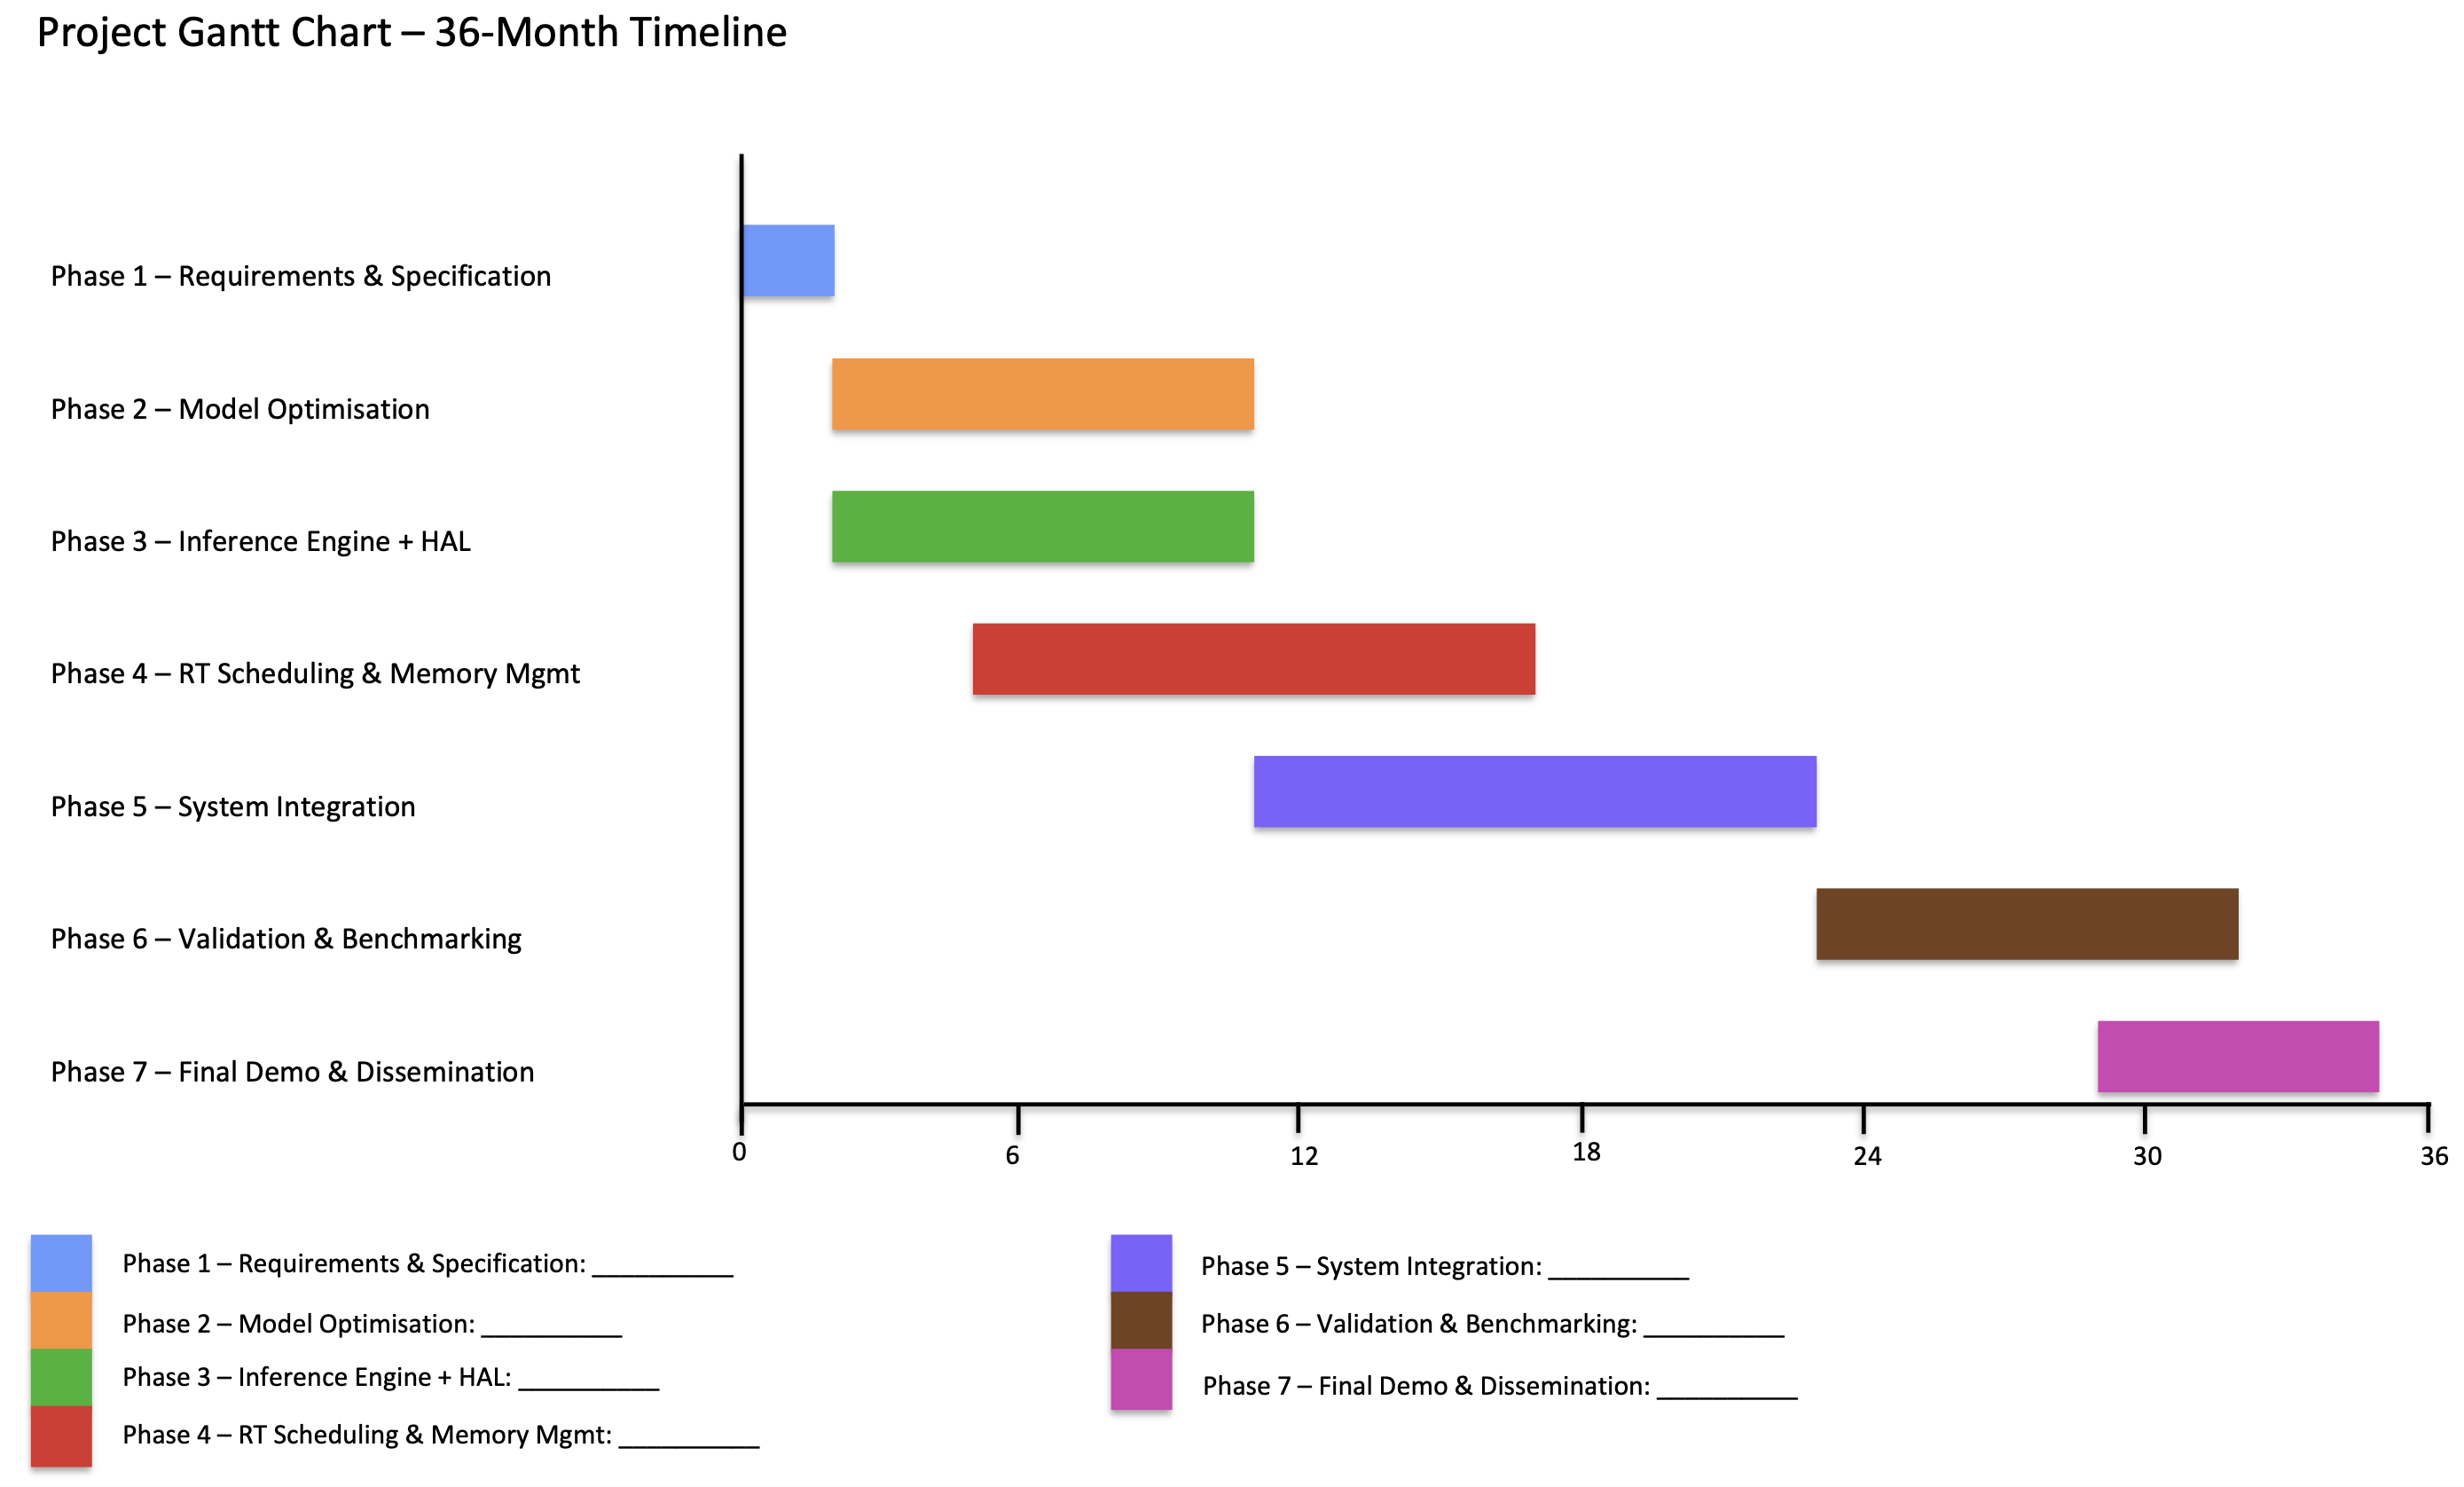
\includegraphics[width=\textwidth]{gantt.png}
  \caption{Project Timeline}
  \label{fig:project_gantt}
\end{figure}

As shown in Figure~\ref{fig:project_gantt}, the Gantt chart provides a clear visual of the project's sequencing, highlighting how different technical phases align with critical milestones and final reporting tasks.



\section{Project feasibility: available resources and research team structure}

\subsection{Existing Resources at the Host Institution}
The host Embedded Systems Laboratory provides an environment purpose-built for TinyML research. Its hardware inventory includes ten STM32F746 Discovery boards offering 320 kilobytes of SRAM and an embedded TFT display, four ESP32-S3 modules with dual Wi-Fi and Bluetooth radios, and a pre-production Arm Cortex-M55 evaluation kit that exposes the Helium SIMD extension. Complementing the microcontroller stock are twelve microphone breakout boards, six high-g accelerometer pods and a vibration test bench derived from an off-the-shelf brushless motor equipped with controllable imbalance weights. A Yokogawa WT500 power analyser and a nano-amp resolution Joulescope add precise energy measurement capability, while a ChipWhisperer-Lite enables fault-injection and side-channel attacks for security audits.

On the software side, the lab maintains a site licence for Keil MDK, both GCC-ARM and LLVM toolchains, the commercial Tracealyzer real-time visualiser and a Jenkins-based continuous-integration cluster that cross-compiles and flashes firmware on demand. Machine-learning workloads run on an on-premises GPU server equipped with four NVIDIA A100 units connected to a high-speed Ceph storage array. A dedicated VLAN and a cloud-linked MQTT broker allow secure remote access for collaborators while isolating experiments from the campus network. The toolchain is compatible with CMSIS-NN primitives~\cite{arm2023cmsislib} and memory mappings defined in Arm's architecture documentation~\cite{arm2023memmodel}.

\subsection{Additional Resources to be Procured}
To stay abreast of commercial silicon roadmaps, the budget allocates funds for two Cortex-M85 evaluation kits that expose the latest Helium-vector instruction set, an Intel MAX-10 field-programmable gate array board used to prototype hardware accelerators and a high-resolution current-sense shield for ultra-low-power sleep profiling. The procurement schedule anticipates six months for silicon availability, so algorithmic work will initially rely on cycle-accurate QEMU simulation. A modest dissemination reserve underwrites open-access publication fees and travel to two flagship conferences in embedded AI and real-time systems. The selected toolchains and platforms will allow firmware integration of CMSIS-NN kernels~\cite{lai2018cmsisnn} and benchmarking of network performance.

\subsection{Project Team and Person-Months}
Project execution will be overseen by an AI Engineer who doubles as Project Manager and contributes eight person‑months distributed across strategic design supervision, milestone planning and risk management. Development of cloud services and data pipelines is handled by a Backend Developer who commits eighteen person‑months to ensure robust APIs and scalable storage. Hardware bring‑up, measurement automation and exploratory FPGA prototyping fall to a part‑time Embedded Engineer working twelve person‑months spread over the first two years. A UI/UX Designer is engaged part‑time, roughly four person‑months as required, to craft intuitive dashboards and mobile interfaces. Quality assurance is provided by a part‑time QA Tester allocating four person‑months to automated regression suites and release validation. Specialised kernel ports or security‑library integrations are undertaken by a Freelance Engineer who supplies six person‑months across critical integration milestones. This compact roster—AI Engineer (Project Manager), Backend Developer, Embedded Engineer (part‑time), UI/UX Designer (part‑time as needed), QA Tester (part‑time) and Freelance Engineer—maintains rapid communication while covering the entire stack from silicon to user experience.


\subsection{Adequacy of Team and Infrastructure}
The infrastructure enumerated above fully covers the technical needs of the project from silicon through toolchains to measurement equipment, allowing immediate commencement without lead-time penalties. All key competencies are represented within the team: neural-network compression, low-level kernel optimisation, real-time system design and applied cryptography. Importantly, skills overlap so that holiday or departure of a single member does not stall progress. A continuous-integration pipeline enforces regression tests, guaranteeing that incremental optimisation never violates functional or security requirements.

Risk is proactively managed. Potential delays in silicon shipping are mitigated by QEMU-based emulation and by maintaining alternate MCU targets. Accuracy loss following aggressive pruning is controlled through quantisation-aware fine-tuning and knowledge distillation. Security regressions are avoided through mandatory code review of crypto patches, and a side-channel test-suite is executed before each milestone. A security policy framework based on 2024 industry best practices~\cite{embedded2024iotsecurity} will guide firmware protection measures. Ten percent contingency is reserved in both time and budget to absorb unforeseeable disruptions.

\subsection{Preliminary Results and Feasibility Evidence}
A series of pre-proposal experiments validate the working hypothesis. On a baseline STM32F746 clocked at two hundred megahertz, an eight-bit quantised and fifty-percent pruned variant of ResNet-18 required only 138 kilobytes of flash and sixty-four kilobytes of SRAM while sustaining ninety-one percent accuracy on CIFAR-10. Kernel-level tuning reduced depthwise-separable convolution latency by a factor of 4.4 and energy per inference by sixty-eight percent compared to unoptimised CMSIS-NN~\cite{lai2018cmsisnn}. A separate proof-of-concept integrated secure boot and encrypted model storage with less than nine percent additional latency. These results mirror optimisations seen in prior keyword-spotting pipelines~\cite{bushur2023keyword}, confirming that the objectives set forth in this proposal are ambitious yet realistic.





\newpage

\section{Risks and alternative approaches}

The following section identifies the main risks that could threaten the smooth execution of the project, assesses their likelihood and impact, and then presents both mitigation strategies and fallback solutions. A modest contingency of time and budget is assumed for each. Risk management principles follow ISO 31000:2018~\cite{iso31000}, with special attention to system-level threats emphasized in NIST SP 800-161 Rev. 1~\cite{nist2022supplychain}.

\subsection{Potential Risks}

Table~\ref{tab:risk_assessment} summarizes the key risks identified at this stage of the project. These risks span technical, logistical, and software-related challenges. Each entry includes a brief description along with an assessment of its likelihood and potential impact on project objectives.

\begin{table}[h]
  \centering
  \begin{tabular}{p{4cm} c c p{6cm}}
    \hline
    \textbf{Risk} & \textbf{Likelihood} & \textbf{Impact} & \textbf{Description} \\
    \hline
    Silicon delivery delays & Medium & High &
      Late arrival of Cortex-M85 or FPGA boards due to supply‐chain issues~\cite{deloitte2021supplychain}. \\
    Accuracy degradation & Low & High &
      Excessive pruning/quantisation causes unacceptable loss of inference accuracy~\cite{krishnamoorthi2018quantizing}. \\
    Integration complexity & Medium & Medium &
      Unforeseen API mismatches between generated kernels and Zephyr RTOS hooks. \\
    Real-time jitter & Low & Medium &
      Variability in inference time undermines deterministic guarantees. \\
    Security vulnerabilities & Low & High &
      Bugs in secure‐boot or encryption routines expose model or firmware~\cite{nist2022supplychain}. \\
    Toolchain obsolescence & Low & Low &
      Deprecation of compiler flags / vendor libraries (e.g.\ CMSIS-NN). \\
    \hline
  \end{tabular}
  \caption{Risk assessment: likelihood and impact}
  \label{tab:risk_assessment}
\end{table}

As shown in Table~\ref{tab:risk_assessment}, even low-likelihood risks such as security vulnerabilities and toolchain deprecations have been considered due to their potentially high impact or long-term effects on maintainability and reliability.

\subsection{Mitigation Strategies and Alternative Approaches}

\begin{itemize}
  \item \textbf{Silicon delivery delays.} 
    \emph{Mitigation:} Start early development on QEMU-based cycle-accurate simulation; maintain dual targets (Cortex-M55, ESP32-S3).  
    \emph{Alternative:} Deploy on readily available boards (e.g.\ STM32F7 series) while awaiting new silicon~\cite{deloitte2021supplychain}.
  
  \item \textbf{Accuracy degradation.} 
    \emph{Mitigation:}  
    \begin{itemize}
      \item Use quantisation-aware fine-tuning and knowledge distillation to recover lost accuracy.
      \item Set dynamic thresholds in the pruning engine to prevent drops below 95\%.
    \end{itemize}
    \emph{Alternative:} Employ hybrid bit-width schemes (e.g.\ 8-bit activations + 4-bit weights) or selective filter pruning~\cite{krishnamoorthi2018quantizing}.
  
  \item \textbf{Integration complexity.} 
    \emph{Mitigation:}  
    \begin{itemize}
      \item Define and validate a stable C API early, with unit tests for each module.
      \item Stage incremental integration in the CI pipeline (kernel, runtime, security).
    \end{itemize}
    \emph{Alternative:} Fall back to a simpler scheduling model (e.g.\ FreeRTOS) if Zephyr hooks prove too brittle.
  
  \item \textbf{Real-time jitter.} 
    \emph{Mitigation:}  
    \begin{itemize}
      \item Perform WCET analysis with static schedulability tools.
      \item Reserve buffer slots in the memory planner to absorb timing spikes.
    \end{itemize}
    \emph{Alternative:} Introduce a lightweight watchdog or a prioritized “heartbeat” task to enforce deadlines.
  
  \item \textbf{Security vulnerabilities.} 
    \emph{Mitigation:}  
    \begin{itemize}
      \item Adopt a strict crypto review process for all bootloader and AES-GCM code.
      \item Automate side-channel tests in the CI before each milestone~\cite{nist2022supplychain}.
    \end{itemize}
    \emph{Alternative:} If hardware crypto engines are unavailable, switch to software implementations with reduced throughput but proven libraries (e.g.\ mbedTLS).
  
  \item \textbf{Toolchain obsolescence.} 
    \emph{Mitigation:}  
    \begin{itemize}
      \item Containerize build environments and archive known-good toolchain versions.
      \item Monitor vendor updates and budget periodic toolchain upgrades.
    \end{itemize}
    \emph{Alternative:} Maintain a minimal fallback using GCC-ARM only, with reduced optimizations.
\end{itemize}

\titlespacing*{\section}
  {0pt}{10pt}{5pt}



  
\section{Impact and dissemination}

\subsection{Scientific Impact}
This endeavor seeks to revolutionize the tailoring of artificial intelligence (AI) models for embedded and edge systems by integrating algorithm development with hardware and software co-design. Such a shift is expected to yield multiple scientific contributions:
\begin{itemize}
  \item \textbf{Novel Co-design Frameworks:} Frameworks will be developed and validated to unify neural architecture search, hardware-aware optimization, and real-time system constraints into a single design loop. These frameworks will push edge AI capabilities far beyond the limitations of sequential design processes.
  \item \textbf{Benchmark Suites:} A comprehensive suite of benchmarks and performance metrics will be released, covering diverse applications like low-latency control, secure inference, and energy-aware sensing. This suite will foster reproducibility and enable rigorous comparisons in future research.
  \item \textbf{Algorithmic Advances:} New compression techniques, dynamic pruning strategies, and ASIP-tailored neural operators will be proposed, each co-optimized for specific hardware characteristics such as custom instructions, memory hierarchies, and power-management units.
  \item \textbf{Toolchain Extensions:} Open-source extensions to widely adopted AI toolchains (e.g., TensorFlow Lite, ONNX Runtime) will incorporate co-design routines for automatic layer scheduling, memory allocation, and integrated security checks.
\end{itemize}
These outcomes will be disseminated through high-impact journals (e.g., IEEE Transactions on Computer-Aided Design, ACM Transactions on Embedded Computing Systems) and flagship conferences (e.g., NeurIPS, ICCAD, ESWEEK), ensuring broad visibility and adoption.

\subsection{Societal and Economic Impact}

The project addresses major challenges at the convergence of AI, embedded systems, and IoT technologies. By enabling efficient AI inference on low-cost microcontrollers, it expands access to smart functionality in domains such as healthcare, environmental monitoring, and assistive devices \cite{Lu2022semi}. This increased accessibility lowers barriers for underserved communities and small enterprises alike.

Optimizing workloads for on-device execution also reduces dependency on centralized cloud services, cutting both energy consumption and data privacy risks. Techniques like energy-aware scheduling and dynamic voltage–frequency scaling are expected to yield system-level savings of up to 50\% in real-world prototypes.

From an economic perspective, the co-design framework supports European industry competitiveness by accelerating integration of embedded AI into next-generation products \cite{Luo2021hscn}. Startups and SMEs can leverage the project’s open-source toolchains to shorten development cycles and reduce costs, contributing to regional innovation ecosystems.

\subsection{Dissemination Strategy}

A multi-faceted dissemination plan will ensure that the project’s outputs reach both academic and industrial stakeholders. Research results will be shared through high-impact journal publications, peer-reviewed conference papers, and invited presentations at major symposia.

All software artifacts—including toolchain extensions, benchmark datasets, and documentation—will be made publicly available under the Apache 2.0 license via a dedicated GitHub organization. Continuous integration pipelines will provide ready-to-use binaries and maintain reproducibility.

To support education and training, teaching materials and laboratory modules will be developed for integration into university courses on embedded AI and system design. Hackathons and summer schools will further engage Master’s and PhD students in hands-on co-design activities.

The project will also organize two industry-focused events to present live demonstrations and collect feedback from semiconductor vendors, OEMs, and system integrators. These engagements will be complemented by technical whitepapers and deployment guidelines.

\subsection{Exploitation and Standardization}

To ensure long-term impact beyond the project duration, several exploitation pathways will be pursued.

Project members will contribute actively to international standardization efforts through ISO/IEC JTC1/SC42 (Artificial Intelligence) and IEEE P2631 (Edge AI). These contributions will help shape best practices and ensure that co-design methodologies inform future standards.

Technical innovations with commercialization potential—such as optimized pruning pipelines or secure scheduling frameworks—will be evaluated for patent protection \cite{Tuli2022codebench}. The university’s technology transfer office will support licensing and spin-off exploration.

Sustainability will be ensured by maintaining open-source repositories after the project’s completion. A documented roadmap will guide future contributions from the community and adaptation to new hardware platforms as they emerge.




\section{Requested budget}

The budget requested for this project is distributed by expense type, necessary roles (Table~\ref{tab:personnel-by-role}) and by project year (Table~\ref{tab:budget-RON}), and is also summarized in Euro at the project level (Table~\ref{tab:budget-eur}). Purchases of any new equipment exceeding 75\,000 RON (price without VAT) are justified with reference to the project objectives. The Project Leader will dedicate a minimum of 20 hours per month to the project.

This budget structure aligns with best practices recommended in the Horizon 2020 Annotated Model Grant Agreement (AMGA)~\cite{ec_amga2020}, particularly regarding proportional allocation to direct and indirect costs, and transparency in staff-role justification.

\subsection{Project Team and Salary Allocation}

To execute the project successfully, we identify the following key roles critical to implementation. These include core engineering, quality assurance, and project management personnel. The salary estimates reflect market rates in Romania for mid-level professionals, and all amounts are presented in RON (1 EUR ≈ 5 RON) over the project's three years.

\vspace{0.5\baselineskip}

\begin{table}[htbp]
  \centering
  \begin{tabular}{p{3.5cm} c c c c}
    \hline
    \textbf{Role} & \textbf{Year I (RON)} & \textbf{Year II (RON)} & \textbf{Year III (RON)} & \textbf{Total (RON)} \\
    \hline
    AI Engineer (Project Manager)            &  50\,000 &  45\,000 &  45\,000 & 140\,000 \\
    Backend Developer                        &  40\,000 &       0  &       0  &  40\,000 \\
    Embedded Engineer (part-time)            &  20\,000 &       0  &       0  &  20\,000 \\
    UI/UX Designer (part-time – as needed)   &   5\,000 &   5\,000 &   5\,000 &  15\,000 \\
    QA Tester (part-time)                    &  10\,000 &   7\,500 &   7\,500 &  25\,000 \\
    Freelance Engineer (as needed, Y2–Y3)    &       0  &  55\,000 &  55\,000 & 110\,000 \\
    \hline
    \textbf{Total Personnel}                 & 125\,000 & 112\,500 & 112\,500 & 350\,000 \\
    \hline
  \end{tabular}
  \caption{Personnel expenses by role and by project year (in RON)}
  \label{tab:personnel-by-role}
\end{table}


As shown in Table~\ref{tab:personnel-by-role}, the largest share of the budget is allocated to core engineering roles, with flexibility built in for freelance support during later phases. Roles listed as part-time or as-needed ensure efficient resource use while maintaining critical coverage.

\subsection{Justification of Major Equipment Purchases}

Any single item with a unit cost above 75\,000 RON (price without VAT) is essential to meet the real-time, low-power inference requirements of our framework:

\begin{itemize}
  \item \textbf{Arm Cortex-M85 evaluation kits} (2 units, \(\sim80\,000\) RON each): needed to tune Helium-accelerated kernels and validate end-to-end energy measurements under real workloads.
  \item \textbf{Intel MAX-10 FPGA board} (\(\sim95\,000\) RON): required for prototyping and verifying custom accelerator blocks in parallel with software co-design.
\end{itemize}

The table below provides a detailed budget breakdown by major cost category across the three years of the project. This includes personnel, logistics, travel, and indirect costs, with equipment expenses highlighted as a key component under logistics.

\vspace{0.5\baselineskip}

\begin{table}[H]
  \centering
  \begin{tabular}{p{3.5cm} c c c c}
    \hline
    \textbf{Budget chapter} & \textbf{Year I (RON)} & \textbf{Year II (RON)} & \textbf{Year III (RON)} & \textbf{Total (RON)} \\
    \hline
    Personnel expenses            & 125 000 & 112 500 & 112 500 & 350 000 \\
    Logistics expenses            &  60 000 &  30 000 &  10 000 & 100 000 \\
    \quad of which equipment      &  50 000 &  20 000 &  10 000 &  80 000 \\
    Travel expenses               &  10 000 &  10 000 &  10 000 &  30 000 \\
    Indirect expenses (overheads) &  40 000 &  40 000 &  40 000 & 120 000 \\
    \hline
    \textbf{Total}                & 235 000 & 192 500 & 172 500 & \textbf{600 000} \\
    \hline
  \end{tabular}
  \caption{Budget distribution by type and by project year (in RON)}
  \label{tab:budget-RON}
\end{table}

\vspace{0.5\baselineskip}

As shown in Table~\ref{tab:budget-RON}, personnel expenses account for the majority of the budget, with capital investment in evaluation hardware captured under logistics. Indirect expenses and travel remain steady across all project years.

For clarity and international transparency, the table below summarizes the total project budget in Euros, using a fixed exchange rate of 1 EUR = 5 RON.

\vspace{0.5\baselineskip}

\begin{table}[H]
  \centering
  \begin{tabular}{p{5cm} c}
    \hline
    \textbf{Budget chapter} & \textbf{Total (EUR)} \\
    \hline
    Personnel expenses            &  70 000 \\
    Logistics expenses            &  20 000 \\
    \quad of which equipment      &  16 000 \\
    Travel expenses               &   6 000 \\
    Indirect expenses (overheads) &  24 000 \\
    \hline
    \textbf{Total}                & \textbf{120 000} \\
    \hline
  \end{tabular}
  \caption{Budget summary at project level (in Euro, 1 EUR = 5 RON)}
  \label{tab:budget-eur}
\end{table}

\vspace{0.5\baselineskip}

Table~\ref{tab:budget-eur} confirms that the overall budget remains within typical bounds for mid-scale research initiatives, with equipment costs carefully justified to support project milestones and funding eligibility criteria aligned with Horizon 2020 guidelines~\cite{ec_amga2020}.
